%%%%%%%%%%%%%%%%%%%%%%%%%%%%%%%%%%%%%%%%%%%%%%%%%%%%%%%%%%%%%%%%%%%%%%%%

%%% LaTeX Template for AAMAS-2026 (based on sample-sigconf.tex)
%%% Prepared by the AAMAS-2026 Program Chairs based on the version from AAMAS-2026. 

%%%%%%%%%%%%%%%%%%%%%%%%%%%%%%%%%%%%%%%%%%%%%%%%%%%%%%%%%%%%%%%%%%%%%%%%

%%% Start your document with the \documentclass command.


%%% == IMPORTANT ==
%%% Use the first variant below for the final paper (including auithor information).
%%% Use the second variant below to anonymize your submission (no authoir information shown).
%%% For further information on anonymity and double-blind reviewing, 
%%% please consult the call for paper information
%%% https://cyprusconferences.org/aamas2026/submission-instructions/


%%%% For anonymized submission, use this
%\documentclass[sigconf,anonymous]{aamas} 

%%%% For camera-ready, use this
\documentclass[sigconf]{aamas} 


%%% Load required packages here (note that many are included already).

\usepackage{balance} % for balancing columns on the final page

%%%%%%%%%%%%%%%%%%%%%%%%%%%%%%%%%%%%%%%%%%%%%%%%%%%%%%%%%%%%%%%%%%%%%%%%

%%% == IMPORTANT ==
%For the final camera-ready submission, you will be assigned a DOI. The DOI suffix is included in the subject line of an email sent by Sheridan, which starts with ``About your submission'' (for example: ``About your submission (aamas LT) … DOI: NIBB4567''). Copy this suffix and paste it into the \verb|\doi| command in the preamble. Do not confuse this with the \verb|\acmDOI| command in the copyright block, which must not be changed. DOIs will be registered and become active shortly after the material is published in the ACM Digital Library (estimated to be on or about the start of the event).

\doi{RGWK4224}

%%%%%%%%%%%%%%%%%%%%%%%%%%%%%%%%%%%%%%%%%%%%%%%%%%%%%%%%%%%%%%%%%%%%%%%%

%%% AAMAS-2026 copyright block (do not change!)

\makeatletter
\gdef\@copyrightpermission{
  \begin{minipage}{0.2\columnwidth}
   \href{https://creativecommons.org/licenses/by/4.0/}{
\includegraphics[width=0.90\textwidth]{by}}
  \end{minipage}\hfill
  \begin{minipage}{0.8\columnwidth}
   \href{https://creativecommons.org/licenses/by/4.0/}{This work is licensed under a Creative Commons Attribution International 4.0 License.}
  \end{minipage}
  \vspace{5pt}
}
\makeatother

\setcopyright{ifaamas}
\acmConference[AAMAS '26]{Proc.\@ of the 25th International Conference
on Autonomous Agents and Multiagent Systems (AAMAS 2026)}{May 25 -- 29, 2026}
{Paphos, Cyprus}{C.~Amato, L.~Dennis, V.~Mascardi, J.~Thangarajah (eds.)}
\copyrightyear{2026}
\acmYear{2026}
\acmDOI{}
\acmPrice{}
\acmISBN{}

%%%%%%%%%%%%%%%%%%%%%%%%%%%%%%%%%%%%%%%%%%%%%%%%%%%%%%%%%%%%%%%%%%%%%%%%

%%% == IMPORTANT ==
%%% Use this command to specify your OpenReview submission number.
%%% In anonymous mode, it will be printed on the first page.

\acmSubmissionID{dm59}

%%% Use this command to specify the title of your paper.

\title{An Agentic Voice-Based Assistant for Interactive Conversation and Guidance in Real-World Environments}

\subtitle{Demonstration Track}

%%%%%%%%%%%%%%%%%%%%%%%%%%%%%%%%%%%%%%%%%%%%%%%%%%%%%%%%%%%%%%%%%%%%%%%%
%%% Authors (EDIT IF NEEDED)
%%%%%%%%%%%%%%%%%%%%%%%%%%%%%%%%%%%%%%%%%%%%%%%%%%%%%%%%%%%%%%%%%%%%%%%%

\author{Donghao HUANG$^{*}$}
\orcid{0009-0005-6767-4872}
\affiliation{
  \institution{Mastercard}
  \city{Arlington, VA}
  \country{United States}}
\email{donghao.huang@mastercard.com}

\author{Monika PANDEY$^{*}$}
\orcid{0000-0003-2385-4052}
\affiliation{
  \institution{Mastercard}
  \city{Pune}
  \country{India}}
\email{monika.pandey@mastercard.com}

% \author{Zhaoxia WANG}
% \orcid{0000-0001-7674-5488}
% \affiliation{
%   \institution{Singapore Management University}
%   \city{Singapore}
%   \country{Singapore}}
% \email{zxwang@smu.edu.sg}

%%%%%%%%%%%%%%%%%%%%%%%%%%%%%%%%%%%%%%%%%%%%%%%%%%%%%%%%%%%%%%%%%%%%%%%%

\begin{abstract}
We present AVA, an agentic, hands-free voice assistant that provides interactive, contextual guidance in real-world environments such as makerspaces. AVA combines large language models with retrieval-augmented generation over environment-specific knowledge (e.g., manuals and safety procedures) and an explicit agent decision/control graph to infer user intent, estimate confidence in retrieved information, and choose dialogue actions such as answering directly, asking clarifying questions, or guiding exploration. The system supports coherent multi-turn interaction via lightweight session memory and augments spoken responses with dynamically generated QR codes linking to authoritative resources. AVA demonstrates real-time, situated assistance for tool discovery, safe operation, and project ideation, highlighting the value of agent-based architectures for scalable, consistent support in evolving physical spaces.
% Many real-world environments provide access to complex tools and technical resources, yet users often struggle to identify appropriate equipment, understand safe operation procedures, and locate relevant documentation. While human assistants can help address these needs, they are not always available, may have limited domain coverage, and cannot scale to continuously answer diverse and evolving user questions across locations and time.

% We present AVA an agentic, voice-based assistant for interactive conversation and contextual guidance in real-world environments, using a Makerspace as a representative deployment scenario. The system integrates large language models with retrieval-augmented generation and an explicit agent decision graph to interpret spoken user input, infer intent, assess confidence in retrieved knowledge, and autonomously decide whether to provide a direct response or request clarification. To support coherent multi-turn interaction, the assistant maintains lightweight session memory, allowing it to leverage prior dialogue context when generating subsequent responses. Interaction is fully speech-based, enabling hands-free use in physical settings. The assistant delivers concise spoken guidance and augments responses with dynamically generated QR codes that link users to authoritative manuals, safety instructions, and supporting resources. The solution showcases a language-enabled, embodied autonomous agent capable of real-time perception–reasoning–action cycles, adaptive dialogue flow, session-aware context handling, and robust decision-making during live interaction in a physical environment.
\end{abstract}

\keywords{Voice Assistant; Agentic Architecture; Situated Interaction}

%%%%%%%%%%%%%%%%%%%%%%%%%%%%%%%%%%%%%%%%%%%%%%%%%%%%%%%%%%%%%%%%%%%%%%%%

\begin{document}

\pagestyle{fancy}
\fancyhead{}

\maketitle

\renewcommand{\thefootnote}{\fnsymbol{footnote}}
\footnotetext[1]{Equal contribution.}
\renewcommand{\thefootnote}{\arabic{footnote}}

%%%%%%%%%%%%%%%%%%%%%%%%%%%%%%%%%%%%%%%%%%%%%%%%%%%%%%%%%%%%%%%%%%%%%%%%
\section{Introduction}
%%%%%%%%%%%%%%%%%%%%%%%%%%%%%%%%%%%%%%%%%%%%%%%%%%%%%%%%%%%%%%%%%%%%%%%%

Physical environments like innovation labs, shared workspaces, and educational makerspaces increasingly depend on diverse tools, procedures, and safety rules. Yet general-purpose voice assistants are not designed for these settings: they lack awareness of local inventories, operational constraints, and context-specific documentation, which limits their usefulness for situated, task-oriented help. At the same time, relying on human staff does not scale---availability varies, expertise may be uneven, and support quality can be inconsistent as toolsets evolve and user questions remain open-ended. Makerspaces illustrate this challenge especially well, since users often struggle to discover the right tools, understand safe operation, and connect documentation across fabrication, robotics, and electronics workflows. To address this gap, we demonstrate\footnote{Demo video available at \url{https://vimeo.com/1153194189}} an agentic, hands-free voice assistant that combines large language models~\cite{openai2023} with retrieval over environment-specific knowledge~\cite{lewis2020rag} and an explicit agent control framework~\cite{wooldridge2009,russell2021}. The agent infers user intent, estimates confidence in retrieved information, and selects dialogue actions such as answering directly, asking clarifying questions, or guiding exploration. It supports coherent multi-turn interaction through lightweight session memory and augments spoken guidance with dynamically generated QR codes linking to authoritative manuals and resources. Overall, the system highlights how agent-based architectures can provide scalable, context-grounded assistance for tool discovery, safe operation, and creative ideation beyond what general-purpose voice technologies can offer.

% Physical environments such as innovation labs, shared workspaces, and educational facilities increasingly rely on diverse tools and workflows. General-purpose voice assistants, while effective in consumer settings, lack awareness of local resources, safety constraints, and operational context, making them unsuitable for situated, task-oriented assistance.

% Users in such environments require contextual guidance for tool discovery, safe operation, and creative exploration. Human assistants face limitations in availability, scalability, and consistency, particularly in spaces that host evolving toolsets and open-ended user curiosity.

% Makerspaces exemplify this challenge by providing heterogeneous fabrication, robotics, and electronics tools that are difficult to navigate without domain-specific support. Users often struggle to identify appropriate tools, combine resources effectively, or reason about feasible projects within the constraints of the space.

% We demonstrate\footnote{Demo video available at \url{https://vimeo.com/1153194189}} an agentic, voice-based assistant for interactive conversation and contextual guidance in real-world environments, using a Makerspace as a representative deployment scenario. The system employs an explicit agent control framework that integrates large language models with retrieval-augmented generation over environment-specific knowledge. The agent autonomously infers user intent, estimates confidence in retrieved information, and selects dialogue actions such as direct response, clarification, or guided exploration.

% Interaction is fully speech-based and hands-free, supported by lightweight session memory for coherent multi-turn dialogue. Responses are augmented with dynamically generated QR codes linking to authoritative manuals and resources. Beyond procedural guidance, the agent supports project ideation and cross-tool brainstorming grounded in available resources.

% The demonstration highlights a language-enabled autonomous agent capable of real-time perception, deliberation, and adaptive dialogue in a physical environment, illustrating the benefits of agent-based architectures for situated assistance beyond general-purpose voice technologies.

%%%%%%%%%%%%%%%%%%%%%%%%%%%%%%%%%%%%%%%%%%%%%%%%%%%%%%%%%%%%%%%%%%%%%%%%
\section{System Overview}
%%%%%%%%%%%%%%%%%%%%%%%%%%%%%%%%%%%%%%%%%%%%%%%%%%%%%%%%%%%%%%%%%%%%%%%%

\begin{figure*}[t]
    \centering
    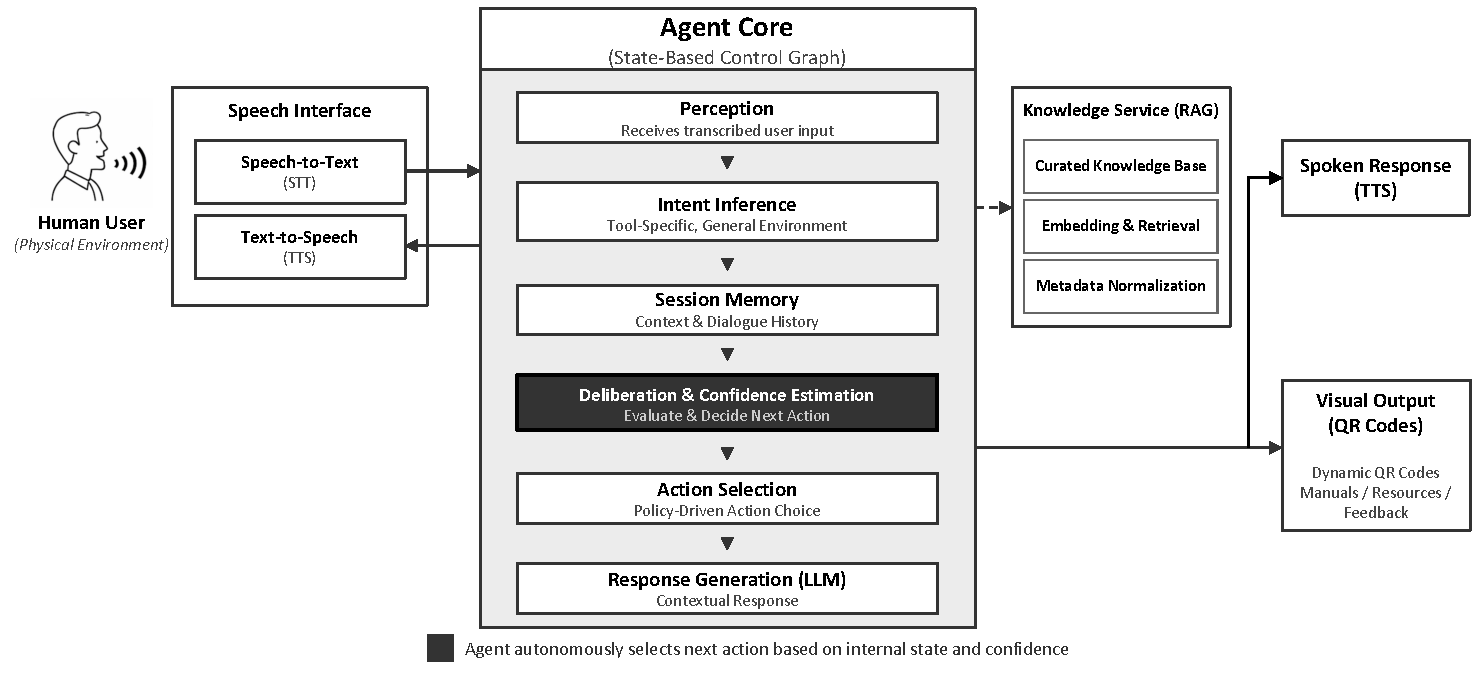
\includegraphics[width=.95\linewidth]{AVA_Architecture.pdf}
    \caption{Agentic architecture of the voice-based assistant.}
    \label{fig:placeholder}
\end{figure*}

\noindent\textbf{Application Scenario.}
The system is deployed as a walk-up kiosk in a Makerspace where users interact via natural spoken queries (e.g., \emph{``What can I do here?''} or \emph{``How do I use the robotic dog?''}). The assistant interprets intent, retrieves environment-specific knowledge, and delivers hands-free spoken guidance, augmented by dynamically generated QR codes linking to manuals and safety documentation. While demonstrated in a Makerspace, the design generalizes to innovation labs, educational facilities, and other instrumented physical environments.

\noindent\textbf{Architecture.}
As shown in Figure~1, the system adopts a modular, agent-centric architecture that separates interaction handling, agent reasoning, knowledge access, and output grounding.
\begin{itemize}
\item \textbf{Speech Interface}: Provides bidirectional voice interaction via speech-to-text and text-to-speech~\cite{speechsurvey}. Continuous listening with silence-based segmentation enables hands-free, walk-up use.

\item \textbf{Agent Core}: Implements autonomous decision-making as an explicit state-based control graph progressing through perception, intent inference, deliberation, and response generation. Utterances are classified into general queries, tool-specific requests, or session termination signals. Lightweight session memory captures dialogue context and salient entities.
A key capability is confidence-aware deliberation: the agent assesses information sufficiency and autonomously selects its next action---direct response, clarification, or redirection---outside the language model, ensuring action selection is governed by agent state rather than model output alone.
\item \textbf{Knowledge Service}: Implements retrieval-augmented generation (RAG) over a curated knowledge base of tool manuals, procedures, and safety guidelines. Retrieved documents are annotated with metadata and injected into the LLM context together with session memory to enable grounded responses.
\item \textbf{Visual Output}: Dynamically renders contextual QR codes linking to referenced tools or resources, providing seamless access to detailed documentation without interrupting the interaction flow.
\end{itemize}


%%%%%%%%%%%%%%%%%%%%%%%%%%%%%%%%%%%%%%%%%%%%%%%%%%%%%%%%%%%%%%%%%%%%%%%%
\noindent\textbf{Agentic Behavior.}
%%%%%%%%%%%%%%%%%%%%%%%%%%%%%%%%%%%%%%%%%%%%%%%%%%%%%%%%%%%%%%%%%%%%%%%%
The system exhibits agentic autonomy through a confidence-aware decision policy. After retrieving candidate knowledge via the RAG service, the agent evaluates evidence sufficiency and maintains an internal confidence estimate. When confidence is high, it produces a grounded response; when low or underspecified, it autonomously initiates clarifying questions. This behavior is realized through state transitions in the agent control graph rather than prompt engineering alone~\cite{embodiedagents}, enabling context-sensitive action selection driven by agent state and environmental knowledge~\cite{situatedinteraction}.

\smallskip\noindent\textbf{Relation to BDI and Neurosymbolic Agent Architectures.}
Recent work has explored combining the principled deliberation of Belief--Desire--Intention (BDI) agents with the natural language capabilities of large language models. ChatBDI~\cite{gatti2025chatbdi}, for instance, adds conversational interfaces to existing BDI agents by translating natural language into KQML performatives, endowing BDI agents with fluent communication while preserving their intentional reasoning. Similarly, other BDI+LLM approaches focus on plan generation~\cite{ichida2024bdi} or goal-directed autonomy within symbolic agent programming frameworks.
AVA's agent control graph shares the BDI commitment to explicit deliberation—intent inference, confidence assessment, and action selection are governed by structured state transitions rather than end-to-end prompting—but differs in two respects. First, AVA targets real-time, situated voice interaction in physical environments, where latency and hands-free usability impose tight constraints on the deliberation cycle. Second, rather than coupling to a full BDI interpreter, AVA adopts a lightweight decision graph that orchestrates an LLM together with RAG retrieval and session memory, balancing interpretability with the flexibility needed for open-ended user queries in evolving physical spaces.

%%%%%%%%%%%%%%%%%%%%%%%%%%%%%%%%%%%%%%%%%%%%%%%%%%%%%%%%%%%%%%%%%%%%%%%
\noindent\textbf{AVA Interaction Flow.}
%%%%%%%%%%%%%%%%%%%%%%%%%%%%%%%%%%%%%%%%%%%%%%%%%%%%%%%%%%%%%%%%%%%%%%%
The live demonstration illustrates an end-to-end user journey, showing how the agent supports exploration, guidance, and feedback in a physical environment:

% \begin{itemize}
(1)~\textbf{Walk-Up Engagement.} 
    A visitor initiates interaction through natural speech at a kiosk. The system automatically establishes a session, enabling continuous, hands-free use without prior setup.

(2)~\textbf{Exploratory Discovery.} 
    Users ask open-ended questions such as \emph{``What can I do here?''}. The agent interprets exploratory intent and provides a concise overview of available tools and activities.

(3)~\textbf{Targeted Guidance.} 
    For tool- or process-specific queries, the agent retrieves environment-specific knowledge and delivers short spoken guidance, emphasizing correct usage and safety.

(4)~\textbf{Contextual Deep-Dive.} 
    When additional detail is relevant, the system displays dynamically generated QR codes linking to official manuals or safety documentation for continued learning.

(5)~\textbf{Adaptive Multi-Turn Dialogue.} 
    The agent maintains lightweight session memory, supporting coherent follow-up questions and adaptive refinement of responses across multiple turns.

(6)~\textbf{Clarification Under Uncertainty.} 
    If a request is ambiguous or insufficiently specified, the agent autonomously asks clarifying questions, demonstrating confidence-aware decision making.

(7)~\textbf{Project Ideation Support.} 
    Beyond procedural assistance, the agent suggests potential projects and tool combinations, encouraging creative exploration aligned with local resources.

(8)~\textbf{Feedback and Session Closure.} 
    At session end, the agent invites user feedback and presents a QR code linking to a feedback form, supporting continuous system improvement.
% \end{itemize}
% 
% \noindent\textbf{AVA Interaction Flow.} The live demonstration showcases an end-to-end user journey through the following stages:
% (1)~\textbf{Walk-Up Engagement}---a visitor initiates interaction via natural speech; the system establishes a session automatically for hands-free use;
% (2)~\textbf{Exploratory Discovery \& Targeted Guidance}---the agent handles both open-ended queries (e.g., \emph{``What can I do here?''}) and tool-specific requests by retrieving environment knowledge and delivering concise spoken guidance;
% (3)~\textbf{Contextual Deep-Dive}---dynamically generated QR codes link to official manuals or safety documentation for continued learning;
% (4)~\textbf{Adaptive Multi-Turn Dialogue \& Clarification}---lightweight session memory enables coherent follow-ups, while confidence-aware deliberation triggers clarifying questions when requests are ambiguous;
% (5)~\textbf{Project Ideation}---the agent suggests projects and tool combinations for creative exploration;
% (6)~\textbf{Feedback \& Closure}---the agent invites feedback via a QR-linked form at session end.

\clearpage
\section{Acknowledgments}
This work was supported by Mastercard Foundry R\&D. The authors thank Varuna Ektare from the Mastercard Foundry Pune R\&D team for her assistance with the program management.
This work was also supported by the EngD Program at Singapore Management University.

\bibliographystyle{ACM-Reference-Format} 
\bibliography{references}

%%%%%%%%%%%%%%%%%%%%%%%%%%%%%%%%%%%%%%%%%%%%%%%%%%%%%%%%%%%%%%%%%%%%%%%%

\end{document}

%%%%%%%%%%%%%%%%%%%%%%%%%%%%%%%%%%%%%%%%%%%%%%%%%%%%%%%%%%%%%%%%%%%%%%%%

